%% ============================================================
%% PAPER E3 -- Edwards Aquifer J-17 forecast evaluation
%% v26 (2026-10-17), continuation of the standalone E3 lineage; v25 is preserved.
%% Base: preserved E3 v25, whose lineage starts at v24 on
%% edwards-framework-e1-audit-implementation. The requested claim-level
%% comparison with Paper11b v2 and Paper11 v67/SI S15--S22 is recorded in
%% PAPER11B_E3_V24_V67_CLAIM_CROSSWALK_2026-10-16.md. Current Paper11 v68
%% alignment/build record: PAPER11B_E3_V25_V68_ALIGNMENT_BUILD_AUDIT_2026-10-17.md.
%% This version preserves v24/v25, keeps the H1/H2 score gate distinct from the
%% broader M2m class clause, and makes no changes to scored results.
%% ============================================================
\documentclass[11pt]{article}
\usepackage[a4paper,margin=1in]{geometry}
\usepackage{amsmath,amssymb,amsthm}
\usepackage{booktabs,longtable,array,tabularx}
\usepackage{graphicx}
\usepackage[hyphens]{url}
\usepackage[colorlinks=true,linkcolor=black,urlcolor=blue,citecolor=blue]{hyperref}
\usepackage[font=small,labelfont=bf]{caption}
\usepackage{placeins}
\usepackage{enumitem}
\setlength{\parskip}{0.45em}
\setlength{\parindent}{0pt}
\setlength{\tabcolsep}{4pt}
\emergencystretch=3em
\newtheorem{proposition}{Proposition}
\newtheorem{remark}{Remark}
\begin{document}

\title{Does a one-pool water-balance model improve forecasts of Edwards Aquifer head? A scored test at J-17}
\author{Amin Abaee\\[0.35em]
{\small Independent Researcher}\\[0.55em]
{\small\href{https://orcid.org/0000-0002-0019-1842}{ORCID: 0000-0002-0019-1842}}\\[0.3em]
{\small\href{mailto:amin\_abaee@ut.ac.ir}{amin\_abaee@ut.ac.ir}}}
\date{October 17, 2026}
\maketitle

{\centering\small \textbf{Prepared in the format of Water Resources Research}\par}
{\centering\small \textbf{Article type: Research Article}\par}

\begin{abstract}
\textbf{Context.} Groundwater maps may fit states better when supplied with future fluxes than can be known at issuance. We test this information-set problem at J-17 in Texas's Edwards Aquifer.

\textbf{Methods.} We score a forward-ordered model ladder against 1934--2023 annual mean daily-high head: 75 rolling one-year origins, 71 five-year origins, and four fixed windows. It includes persistence, training mean, AR(1), one-pool flux maps, residual/delay variants, one-step climate-informed recharge, and a realized-flux diagnostic. The H1/H2 point rule is distinguished from a separate M2m class restriction. The protocol was frozen and archived before scoring, not prospectively registered.

\textbf{Results.} Using previous-year fluxes, the map loses to persistence at one year (14.70 vs 13.23\,ft); with realized target-year fluxes it scores 7.55\,ft, but only as a conditional retrospective diagnostic. AR(1) improves by 0.39\,ft, with an uncertainty interval spanning zero. M2m scores 12.28\,ft and passes H1/H2, but its affine AR(1) reduction is not counted as distinct process structure. Three climate variants pass the M1/persistence point comparator by 0.02--0.13\,ft but are class-demoted; the best paired margin is uncertain. Their five-year scores reuse a one-step recharge forecast. At five years the training mean beats persistence in this record (16.80 vs 21.11\,ft).

\textbf{Conclusions.} The persisted-flux map's failure reflects origin-time driver information, not evidence of structural invalidity. Results describe this record and protocol; annual-mean scores do not establish an operational recommendation for the EAA's 10-day trigger or other aquifers.
\end{abstract}

\textbf{Keywords:} Edwards Aquifer; J-17 index well; groundwater forecasting; water balance; out-of-sample evaluation; persistence; forecast information set.

\textbf{Article Impact Statement.} The one-pool map using last year's recharge does not beat persistence on annual J-17 means. Better scores with realized future fluxes are retrospective diagnostics, not forecasts; score rules and model-class judgments remain distinct.

\section{Introduction}

Forecasts of groundwater head at index wells inform drought monitoring, pumping rules, and ecological-service planning. The statistical target, however, is not always the policy target: an annual mean at a representative well may differ from the subannual statistic used by an agency to activate a restriction. A forecast-evaluation design should therefore state both the measured predictand and the decision statistic it only approximates.

The Edwards (Balcones Fault Zone) Aquifer offers a useful case for examining this distinction. The San Antonio Pool is monitored at J-17, and the Edwards Aquifer Authority (EAA) uses a Stage-I critical-period trigger based on a 10-day running mean below 660\,ft at J-17; the rule came into force in 2007. A level near 618\,ft is often cited as an approximate range at which Comal Springs approaches cessation. We treat the former as an institutional threshold and the latter as a contextual, approximate service level, not as a precisely identified physical barrier. Figure~\ref{fig:j17-series} shows the annual series and these context lines; neither threshold is fitted as a forecast target in the primary evaluation.

\begin{figure}[htbp]
\centering
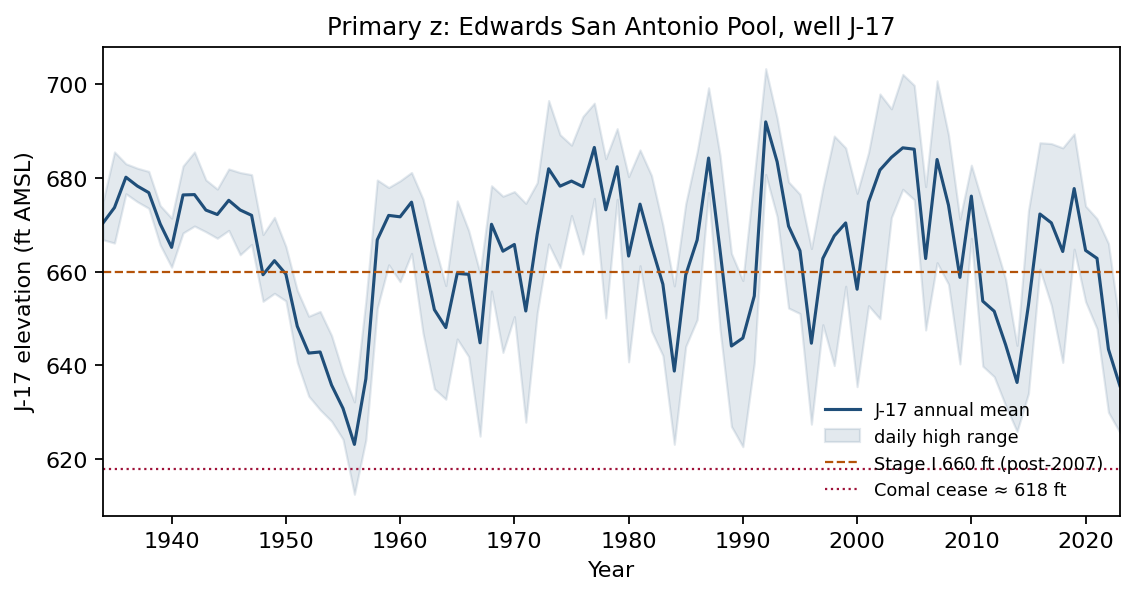
\includegraphics[width=\textwidth]{figs/edw_fig1_series}
\caption{J-17 annual mean of daily-high elevations and the observed annual range (1934--2023). The 660-ft line is the EAA Stage-I threshold, effective from 2007 and defined on a 10-day running mean rather than this annual predictand. The approximate 618-ft Comal cessation level is contextual, not a fitted barrier.}
\label{fig:j17-series}
\end{figure}

Groundwater-level forecasting spans statistical autoregressions, neural networks, lumped water balances, and spatially distributed numerical models (Daliakopoulos et al., 2005; Adamowski and Chan, 2011; Scanlon et al., 2003). Recent benchmark datasets and model comparisons have improved the basis for reproducible comparisons (Ohmer et al., 2026; Zhu et al., 2026). Here the question is narrower than a general contest among algorithms: when an increment model depends on recharge and pumpage that are not known for the target year, does its forecast add skill beyond simple baselines under an explicitly declared information set?

The one-pool map examined here is a discrete-time increment model, not a closed mass-conserving groundwater balance. It approximates annual head change as a linear function of recharge, pumpage, and current head, with a numerical clip. Its coefficients are estimated by least squares within each training window. The empirical question is therefore one of forecast performance, not proof of hydrogeological closure or causal effect.

This article makes three bounded contributions. First, it reports a rolling-origin and fixed-window comparison of the one-pool map and its structural variants against persistence, the training mean, and an AR(1), on the same origins. Second, it states the protocol and separates the point-score rule from a separate class-based decision about whether M2m represents a distinct process model. Third, it derives an exact increment-error identity that separates driver substitution from the residual of a supplied mechanism, then uses the J-17 results to show why a good conditional map need not be a useful origin-time forecast. The study is a single-system evaluation; it does not claim that these score rankings hold for groundwater models or aquifers generally.

A separate Northern cod forecast study uses its own data, protocol, and results (Abaee, 2026). It is not a replication of the J-17 evaluation, and no scores are pooled or transferred between systems.

\section{Data and evaluation design}

\subsection{Predictand, drivers, and thresholds}

The predictand is the calendar-year arithmetic mean of daily-high J-17 head (TWDB well 6837203; EAA well AY-68-37-203), in feet above mean sea level, for 1934--2023. The panel contains 90 annual values. All available daily highs are used; no year falls below the 240-observation rule (the minimum is 242 in 1939), missing days are not interpolated, the published pre-continuous composite is retained as issued, and the 2023 value is provisional. These choices preserve the published observational record; they do not turn the annual average into the EAA's 10-day trigger statistic.

Annual recharge \(R_t\) is the USGS San Antonio-area estimate based on the stream-loss method (Puente, 1978; Umphres and Choi, 2025), in \(10^3\) acre-ft per year. Annual pumpage \(P_t\) is from EAA Table 1. These are regional flux estimates, not direct measurements of storage at J-17; the mapped recharge and pumpage totals include aggregation across the San Antonio and Uvalde areas. Comal Springs discharge \(Q_t\) is taken from USGS station 08168710 and is treated as a secondary service series, not a driver in the head forecast equations. Climate predictors are September--November Niño 3.4 anomalies and calendar-year precipitation in Texas climate divisions 06 and 07. For a forecast issued at December 31 of year \(t\), inputs dated through \(t\) may be used; target-year fluxes are unavailable.

The EAA Stage-I threshold is a 10-day mean below 660\,ft and applies from 2007 onward. We report an annual-mean indicator only as a coarse secondary diagnostic on post-2007 origins; it is not a direct test of the operational rule. The approximately 618-ft Comal level is likewise contextual: observed spring cessation occurred during the 1956 drought, when J-17's annual mean was 623.15\,ft and daily minimum 612.51\,ft. We do not treat 618\,ft as a validated universal barrier.

\subsection{Model ladder}

The fitted one-pool map is
\begin{equation}\label{eq:pool}
H_{t+1}=\left[H_t+\alpha+\beta\widetilde R_{t+1}+\gamma\widetilde P_{t+1}+\delta H_t\right]_{[610,710]},
\end{equation}
where \([\cdot]_{[610,710]}\) clips the forecast to the stated numerical range in feet. The clip is a modeling convention; it is not an empirically identified storage floor. The coefficients are refitted by ordinary least squares on the training transitions at each origin.

The rolling ladder is:
\begin{itemize}[leftmargin=1.5em]
\item \textbf{persist}: \(\widehat H_{t+h}=H_t\), the no-change forecast;
\item \textbf{mean}: the training-window mean of \(H\), recomputed at each origin;
\item \textbf{M1}: an output-only AR(1), \(H_{t+1}=a+\varphi H_t\);
\item \textbf{M2}: the one-pool map with \((\widetilde R,\widetilde P)=(R_t,P_t)\), held at the latest values for multi-step forecasts;
\item \textbf{M2m}: the same map supplied with training-window mean fluxes \((\bar R,\bar P)\);
\item \textbf{M3}: M2 with an autoregressive residual correction;
\item \textbf{M4}: a one-year delayed-state control, included as a theoretical information-lag variant;
\item \textbf{M2\_Rar, M2\_Renso, M2\_Rprecip, M2\_combo}: M2 variants in which recharge is forecast from an AR(1), lagged Niño 3.4, lagged climate-division precipitation, or their combination. For \(h>1\), the one-step recharge forecast is held fixed;
\item \textbf{M2\_oracle}: the same map supplied with realized target-year recharge and pumpage. It is a retrospective conditional diagnostic and is excluded from retention.
\end{itemize}

Under constant climatological fluxes, M2m reduces algebraically to an affine function of current head, \(H_{t+1}=a'+\varphi'H_t\), in the same forecast-function class as an AR(1). Its estimator differs because its intercept is built from the fitted flux terms. This class equivalence is relevant to interpretation, not a change to its observed RMSE.

\subsection{Scoring protocol}

The primary score is rolling-origin RMSE of annual-mean J-17 head. Each model uses the same expanding origin set, with a minimum of 15 training years: \(n=75\) at \(h=1\) and \(n=71\) at \(h=5\). Four fixed historical windows are diagnostic rather than retention tests: drought drawdown (train 1934--1950, test 1951--1956), drought recovery (1934--1956 / 1957--1961), pre-permit wet period (1980--1990 / 1991--1995), and critical-period era (1997--2014 / 2015--2023). The primary evaluation protocol was frozen and archived on 2026-08-25 before its RMSE tables were computed. It is a frozen computational protocol, not a prospective registration.

The score rule, stated in terms of the rolling \(h=1\) point RMSE, requires a candidate to beat both persistence (H1) and its next-simpler candidate (H2). M1 has no simpler process candidate, so H2 is not applicable. Diagnostic-only oracle runs and the Comal service series do not enter retention. The broader frozen protocol document also contains a class-based restriction for M2m; that restriction is not part of the H1/H2 score rule. Therefore we report two decisions separately: whether a model passes the point-score rule, and whether it is counted as a distinct process-structured success. M2m passes H1 and H2 but is not counted as a distinct process-structured result because of its affine AR(1) class reduction. This is a classification choice in the broader protocol, not a statistical failure or an exception to its RMSE.

The climate pass uses M1 as the next-simpler comparator, as stated in its frozen specification, and also reports persistence and M2m as nested baselines. A sign-hit score listed in an earlier design iteration was struck; no result from it is used. Secondary summaries include MAE, uncertainty on paired score differences, and a post-2007 Brier score for the annual-mean indicator below 660\,ft. Since the statutory trigger is based on a 10-day mean, the Brier score is only a coarse proxy.

\section{Results}

\subsection{Primary rolling-origin performance}

Table~\ref{tab:primary} shows the principal scores, and Figure~\ref{fig:j17-rmse} displays the horizon-specific comparisons. At one year M2 (14.70\,ft) is worse than persistence (13.23\,ft); M3 and M4 are also worse than persistence. M1's RMSE is 12.84\,ft, an improvement of 0.39\,ft over persistence, but its MAE is effectively tied (10.72 versus 10.73\,ft), and its paired 95\% moving-block interval for the RMSE margin spans zero. M2m has the lowest point RMSE at one year (12.28\,ft); it beats persistence and M1 and therefore passes H1/H2. It is nevertheless not counted as a distinct process-structured success under the separate class restriction described above. At five years, the training mean scores 16.80\,ft, compared with 21.11\,ft for persistence, 21.25\,ft for M1, and 33.49\,ft for M2. The realized-flux diagnostic is not included in those retention decisions.

\begin{table}[htbp]
\centering\small
\caption{Rolling-origin RMSE (ft) and point-rule reading. All candidate models use identical origins. The M2m class restriction is separate from H1/H2.}
\label{tab:primary}
\begin{tabularx}{\textwidth}{@{}XrrX@{}}
\toprule
Model & \(h=1\) & \(h=5\) & H1/H2 and interpretation \\
\midrule
Persistence & 13.23 & 21.11 & Reference baseline \\
Training mean & 16.17 & \textbf{16.80} & Reference baseline \\
M1 AR(1) & 12.84 & 21.25 & H1 passes; H2 not applicable; margin within uncertainty \\
M2 persisted fluxes & 14.70 & 33.49 & H1 fails \\
M2m climatological fluxes & \textbf{12.28} & 17.44 & H1 and H2 pass; separate class restriction applies \\
M3 residual correction & 14.46 & 33.46 & H1 fails \\
M4 delayed-state control & 14.30 & 33.39 & H1 fails \\
M2 oracle, realized \(R,P\) & 7.55 & 10.86 & Excluded: future inputs \\
\bottomrule
\end{tabularx}
\end{table}

\begin{figure}[htbp]
\centering
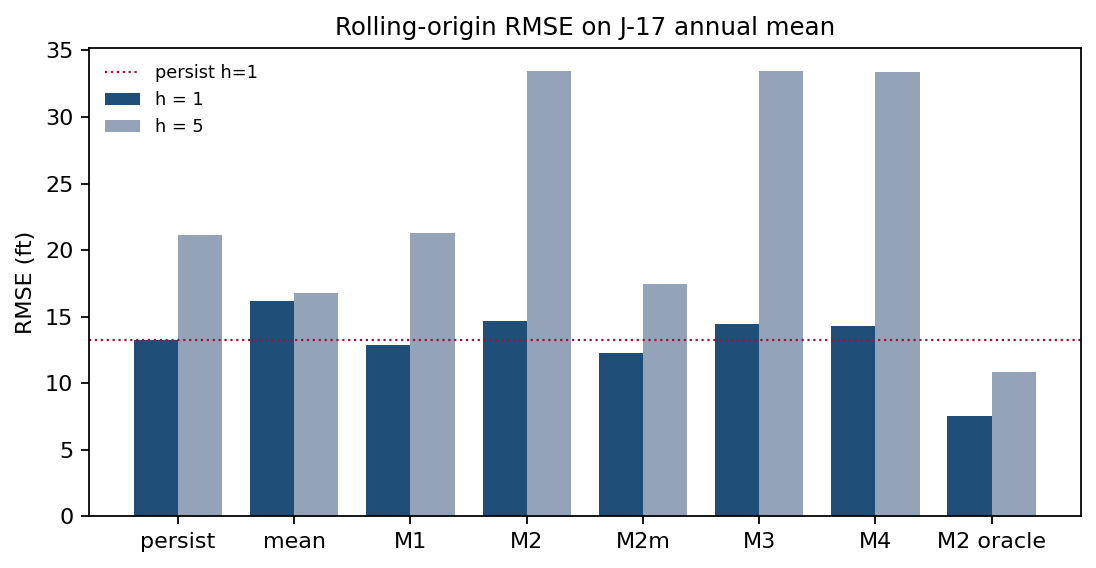
\includegraphics[width=\textwidth]{figs/edw_fig3_rmse}
\caption{Rolling-origin RMSE for annual-mean J-17 head at $h=1$ and $h=5$. The dotted reference line marks $h=1$ persistence (13.23\,ft) and is not the five-year comparator; five-year persistence is 21.11\,ft. The realized-flux conditional diagnostic uses information unavailable at the forecast origin and is excluded from retention.}
\label{fig:j17-rmse}
\end{figure}

The post-freeze uncertainty layer gives a 95\% moving-block interval of \([-1.51,+0.71]\)\,ft for the one-year M1-minus-persistence margin, with Diebold--Mariano \(p=0.40\); an independent implementation reports an interval of \([-1.22,+0.56]\)\,ft and \(p=0.38\). The M2m advantage over persistence is the only one-year margin that clearly separates from zero in both implementations (primary \(p=0.003\), independent \(p=0.001\)). The five-year mean-minus-persistence margin is \(-4.30\)\,ft; its block interval excludes zero and the independent replication gives \(p=0.035\). These inferential summaries concern the scored origins and do not remove the single-system, annual-mean scope.

\subsection{Climate-informed recharge}

The climate variants score between 12.71 and 13.25\,ft at one year, compared with 12.84\,ft for M1 and 12.28\,ft for M2m. Under the documented Pass-2 point comparator (persistence and M1), M2\_Renso, M2\_Rprecip, and M2\_combo are numerically below both comparators; M2\_Rar fails the persistence comparison. The three point-rule margins over M1 are small (0.02--0.13\,ft), and the best, M2\_combo, is not separated from zero (95\% block interval \([-1.37,+1.31]\)\,ft; \(p=0.83\)). The archived code lists these three under the strict point rule, then class-demotes them as M2m-plus-intercept variants rather than additional head-forecast structure. Thus the combined paper's ``no distinct process structure retained'' disposition is a broader structural/classification decision, not failure of the H1/H2 point gate: with M1 as comparator, three are listed and then demoted; with M2m as comparator, none clears the point comparison. At five years the variants score 24.42--26.88\,ft, as the one-step recharge forecasts are held fixed over the horizon; these are not multi-year climate tests. We report the point-gate and class-based dispositions separately, treating uncertainty and five-year performance as interpretation rather than retroactive gate criteria. No statistically supported distinct climate gain is established. Same-year precipitation is not available at the forecast origin; it is reported only as a conditional diagnostic. The full fixed-window and recharge-target scores are in Supplementary Section S11.

\begin{table}[htbp]
\centering\small
\caption{Climate-informed recharge variants. Head RMSE is in feet; recharge RMSE is in \(10^3\) acre-ft. Margins at \(h=1\) are relative to M1.}
\label{tab:climate}
\begin{tabularx}{\textwidth}{@{}Xrrrr@{}}
\toprule
Model & \shortstack{Head RMSE\\$h=1$} & \shortstack{Margin\\vs M1} & \shortstack{Head RMSE\\$h=5$} & \shortstack{Recharge RMSE\\$h=1$} \\
\midrule
M1 & 12.84 & --- & 21.25 & --- \\
M2\_Rar & 13.25 & +0.41 & 25.38 & 561 \\
M2\_Renso & 12.82 & -0.02 & 24.42 & 528 \\
M2\_Rprecip & 12.80 & -0.04 & 25.38 & 545 \\
M2\_combo & 12.71 & -0.13 & 26.88 & 538 \\
M2m climatological fluxes & 12.28 & -0.56 & 17.44 & --- \\
Precipitation diagnostic & 10.56 & --- & 16.91 & 354 \\
\bottomrule
\end{tabularx}
\end{table}

\subsection{Post-freeze service and pumpage diagnostics}

Two analyses were conducted after the retention decision and do not change it. First, Comal Springs discharge is highly correlated with J-17 head over the full record (\(r=0.986\)); a linear rating curve fitted on 1934--1950 predicts about 97\,cfs at the 1956 annual mean, compared with an observed annual mean near 32\,cfs and cessation during part of that drought. This makes the series a useful service diagnostic but not an independent forecast-information source for J-17, and the near-linear rating curve does not resolve the spring's drought-tail threshold behavior. The full same-origin score set and rating-curve caveats are in Supplementary Section S9.

Second, a post-freeze scenario analysis passes alternative pumpage paths through the short pre-permit map fitted on 1980--1990, initialized at the observed 1990 head and forced with realized historical recharge over 1991--2023. The projected 2023 values span 630.9--646.8\,ft, while the map's own scenario RMSEs are 7.19--14.22\,ft. Because the paths use realized recharge, the map is short-window fitted, and its pumpage coefficient is simultaneity-contaminated, these outputs are model-conditioned scenarios, not forecasts or estimates of policy effects. No management recommendation follows from them; the full table and caveats are in Supplementary Section S10.

\section{A decomposition of increment-forecast error}

The model ladder forecasts a state increment using a mechanism evaluated at either a forecast-time substitute for the driver or, in the diagnostic oracle, the realized driver. The difference between those two information conditions can be stated without a distributional or stationarity assumption.

\begin{proposition}[Increment-forecast error identity]\label{prop:increment}
Let \(\Delta_{t+1}=H_{t+1}-H_t\) and suppose a one-step mechanism can be written \(\Delta_{t+1}=m(x_{t+1})+u_{t+1}\), where \(x_{t+1}\) is the target-year driver vector and \(u_{t+1}\) is the residual under that representation. A forecast issued at \(t\) uses a substituted value \(\widehat x_{t+1}\) and predicts \(\widehat\Delta_{t+1}=m(\widehat x_{t+1})\); persistence predicts zero increment. Define \(d_{t+1}=m(x_{t+1})-m(\widehat x_{t+1})\). If the relevant second moments exist, then
\begin{equation}\label{eq:increment}
\mathbb{E}\left[(\Delta_{t+1}-\widehat\Delta_{t+1})^2\right]-\mathbb{E}\left[\Delta_{t+1}^2\right]
=\mathbb{E}[d_{t+1}^2]-\mathbb{E}[m(x_{t+1})^2]-2\mathbb{E}\left[u_{t+1}m(\widehat x_{t+1})\right].
\end{equation}
The same identity holds for empirical mean squared errors when expectations are replaced by averages over a common set of origins.
\end{proposition}

\emph{Proof.} The mechanism forecast error is \(u_{t+1}+d_{t+1}\), whereas the persistence error is \(m(x_{t+1})+u_{t+1}\). Expanding the difference of their squared errors gives \(d^2-m^2+2u(d-m)\). Since \(d-m=-m(\widehat x)\), the cross-term is \(-2u m(\widehat x)\), which yields \eqref{eq:increment}. \(\square\)

For M2, the substitute is the previous year's flux vector. In the scored record, recharge has lag-one autocorrelation 0.17, while the correlation between the head increment and same-year recharge is 0.74; the correlation between the increment and the previous year's recharge is 0.06. These are descriptive record statistics. They are consistent with the M2 result: the map's mechanism is strongly associated with the increment when the target-year flux is supplied, but previous-year recharge carries little of that contemporaneous information. The M2 oracle's 7.55-ft RMSE is therefore evidence about conditional map performance, not about what an origin-time forecast can know. Across the 75 one-year origins, the archived application of the identity attributes +76.03\,ft$^2$ to driver substitution and $-27.49$\,ft$^2$ to the residual cross-term, for an unclipped M2-minus-persistence MSE gap of +48.54\,ft$^2$; the output clip changes the scored gap to +40.99\,ft$^2$ (Supplementary Section~S6). The decomposition also prevents the opposite overreach: a low oracle error does not by itself establish that the map is physically complete, since the residual term includes all omitted processes and measurement error.

\section{Discussion}

\subsection{What the evaluation establishes}

The central result is information-set dependent. M2's persisted-flux forecast is worse than persistence; the same fitted map scores substantially better when supplied with realized target-year fluxes. The increment identity gives a direct way to describe this contrast, while keeping map adequacy separate from the predictability of its inputs. Three origin-available climate variants numerically improve on M1 by 0.02--0.13\,ft under the frozen Pass-2 point gate, but the best margin is unresolved, all three score worse than M2m, and the broader class assessment treats them as M2m-plus-intercept variants rather than additional head-forecast structure. The result is therefore no supported, distinct climate gain—not zero point-score differences. This is a result about this annual J-17 series, this model ladder, and the stated forecast origin.

The point-score decision and the statistical evidence should also remain distinct. M1 passes the point H1 comparison by 0.39\,ft, but its margin is small relative to paired uncertainty and its five-year ordering reverses. M2m has the best one-year point score and passes H1/H2; the separate class restriction means it is not counted as a distinct process-structured improvement. Reporting both facts is preferable to describing M2m as either a score-rule failure or unqualified evidence for a superior water-balance mechanism.

\subsection{Decision thresholds and service relevance}

The annual mean of daily highs is not the EAA's 10-day running mean. Accordingly, the post-2007 Brier score can describe threshold classification on the annual proxy but cannot validate a Stage-I alert system. A policy-facing evaluation would need the same 10-day target, information available at each operational decision date, and a protocol matched to the authority's update cycle. The approximate Comal cessation level is contextual rather than a calibrated barrier in this paper; the 1956 rating-curve failure is a warning against using a near-linear relation at ordinary heads as a drought-tail model.

\subsection{Pumpage scenarios and limits of interpretation}

The post-freeze pumpage exercise is deliberately separate from forecast scoring. It replays observed recharge through a short-window fitted map under alternative pumpage paths; it does not estimate the causal effect of a policy, and the fitted pumpage coefficient is subject to simultaneity because pumping responds to hydrologic conditions. The spread of simulated heads is similar in scale to the map's error, which limits the precision of the scenario comparison. These facts make the exercise useful as a sensitivity illustration, not as evidence that pumping controls are ineffective or that one policy is preferred.

\subsection{Scope and transferability}

The sample is one index well in one managed aquifer, observed at annual resolution. The study does not establish a general ranking for process-based, statistical, or machine-learning groundwater models; it does not infer sustainability, causal pumping effects, or a physical storage volume from head; and it does not identify a universal 618-ft failure barrier. Results may motivate comparable, information-set-explicit evaluations elsewhere, but transfer requires new data, model specification, origin-time constraints, and validation against the relevant management target.

\section{Conclusions}

On the J-17 annual-mean record, the one-pool map supplied with previous-year recharge and pumpage does not improve on persistence at one year. Its much lower error when supplied with realized future fluxes is a conditional diagnostic, not a forecast. The AR(1)'s 0.39-ft point improvement is not distinguishable from zero in the paired uncertainty layer. M2m produces the lowest one-year RMSE and passes the stated H1/H2 score rule, but a separately documented class restriction prevents treating its affine AR(1) reduction as a distinct process-structured success. Three climate-informed variants also pass the M1/persistence point comparisons by 0.02--0.13\,ft; the archived analysis then classifies them as M2m-plus-intercept variants, not additional head-forecast structure. Their best margin is not distinguishable from zero, and their five-year scores reuse a one-step recharge forecast rather than test multi-year climate prediction. We report these as point-rule passes but not distinct, supported climate gains. At five years the training mean beats persistence on these rolling origins; this is not, by itself, a strategic-planning recommendation.

The practical implication is methodological: a groundwater forecast claim should identify its origin-time information set, score against appropriate simple baselines, and separate statistical performance from class or policy interpretation. Because this study forecasts annual means rather than the EAA's 10-day Stage-I statistic, it does not directly establish operational trigger performance. A direct management evaluation would require a target-aligned design and cannot be inferred from the present annual results.

\section*{Data and code availability}

The J-17 annual panel and archived model outputs are held with the Edwards forecast analysis at `wave\_e\_edwards/`; the USGS recharge data release is Umphres and Choi (2025), DOI 10.5066/P1BI62NY; pumpage is from EAA Table 1; Comal discharge is USGS station 08168710; the climate sources are NOAA PSL HadISST and NCEI nClimDiv. The archived analysis panel is the dataset of record for scored results. The nClimDiv raw file is not redistributed; the provenance URL and its three panel columns are recorded, and scoring from the archived analysis panel does not require that raw file. The primary uncertainty analysis and independent replication, the pumpage-scenario script, fixed-window results, and protocol record are described in Supplementary Sections S1--S11. This version does not claim a fresh rerun of the archived forecasting pipeline.

\small
\section*{References}

Adamowski, J., and Chan, H.F. (2011). A wavelet neural network conjunction model for groundwater level forecasting. \emph{Journal of Hydrology}, 407, 28--40. \url{https://doi.org/10.1016/j.jhydrol.2011.06.013}.

Abaee, A. (2026). \emph{Does a surplus-production ladder improve forecasts of Northern cod? A scored test on NAFO 2J3KL}. Zenodo. \url{https://doi.org/10.5281/zenodo.22553609}.

Daliakopoulos, I.N., Coulibaly, P., and Tsanis, I.K. (2005). Groundwater level forecasting using artificial neural networks. \emph{Journal of Hydrology}, 309, 229--240. \url{https://doi.org/10.1016/j.jhydrol.2004.12.001}.

Diebold, F.X., and Mariano, R.S. (1995). Comparing predictive accuracy. \emph{Journal of Business \& Economic Statistics}, 13, 253--263. \url{https://doi.org/10.1080/07350015.1995.10524599}.

Edwards Aquifer Authority (2024). \emph{2023 Groundwater Discharge and Usage}, Table 1. \url{https://www.edwardsaquifer.org/wp-content/uploads/2025/05/2023-Groundwater-Discharge-and-Usage.pdf}.

Edwards Aquifer Authority. Critical Period / Drought Management. \url{https://www.edwardsaquifer.org/groundwater-users/critical-period-drought-management/}.

Künsch, H.R. (1989). The jackknife and the bootstrap for general stationary observations. \emph{Annals of Statistics}, 17, 1217--1241. \url{https://doi.org/10.1214/aos/1176347265}.

Makridakis, S., Spiliotis, E., and Assimakopoulos, V. (2020). The M4 Competition: 100,000 time series and 61 forecasting methods. \emph{International Journal of Forecasting}, 36, 54--74.

National Centers for Environmental Information. NOAA nClimDiv precipitation data. \url{https://www.ncei.noaa.gov/pub/data/cirs/climdiv/}.

NOAA Physical Sciences Laboratory. Niño 3.4 monthly SST (HadISST). \url{https://psl.noaa.gov/data/timeseries/month/data/nino34.long.data}.

Ohmer, M., Liesch, T., Habbel, B., Heudorfer, B., Gomez, M., Clos, P., Nölscher, M., and Broda, S. (2026). GEMS-GER: A machine-learning benchmark dataset of long-term groundwater levels in Germany with meteorological forcings and site-specific environmental features. \emph{Earth System Science Data}, 18, 77.

Puente, C. (1978). \emph{Method of estimating natural recharge to the Edwards Aquifer in the San Antonio area, Texas}. U.S. Geological Survey, Austin, Texas.

Ropelewski, C.F., and Halpert, M.S. (1986). North American precipitation and temperature patterns associated with the El Niño/Southern Oscillation (ENSO). \emph{Monthly Weather Review}, 114, 2352--2362.

Scanlon, B.R., Mace, R.E., Barrett, M.E., and Smith, B. (2003). Can we simulate regional groundwater flow in a karst system using equivalent porous media models? Case study, Barton Springs Edwards aquifer, USA. \emph{Journal of Hydrology}, 276, 137--158.

Texas Water Development Board. Water Data for Texas, well 6837203 (J-17). \url{https://waterdatafortexas.org/groundwater/well/6837203}.

Umphres, G.D., and Choi, N.J. (2025). Estimated annual recharge to the Edwards Aquifer in the San Antonio area, by stream basin or ungaged area, 1934--2024. U.S. Geological Survey data release. \url{https://doi.org/10.5066/P1BI62NY}.

U.S. Geological Survey. National Water Information System, site 08168710, Comal Springs at New Braunfels, Texas.

Zhu, Q., Zhu, Y., Niu, J., Huang, J., Huang, F., Zhou, X., Liu, D., and Hu, B.X. (2026). Benchmarking machine learning and deep learning models for groundwater level prediction in karst aquifers: the dominant role of hydrogeological complexity. \emph{Water}, 18(8), 939. \url{https://doi.org/10.3390/w18080939}.

\normalsize
\section*{Declarations}
\textbf{Funding and competing interests.} None declared.

\textbf{Author contributions.} Amin Abaee: conceptualization, data curation, formal analysis, investigation, methodology, software, validation, visualization, writing---original draft, writing---review and editing.

\textbf{Use of generative AI.} Tools assisted with language editing, register review, and consistency checks. The author checked scientific statements, numbers, protocol events, and conclusions against cited data and archived records.

\end{document}
